\section{Verteilung}
\subsection{Effizienz}
Pareto-Effizienz: Eine wirtschaftspolitische Massnahme ist dann effizient wenn sie die Sitatuion eines Einzelnen verbessert, ohne andere schlechter zu stellen. 
\subsection{Verteilung}
Die Einkommensverteilung hängt ab von der Produktivität der Arbeitenden. Daher verdienen weniger leistungsfähige wenig. Will die Gesellschaft dies nicht aktzeptieren, so muss umverteilt werden.\\
Wird zuviel umverteilt gibt es weniger Anreize zur persönlichen Leistung. Wird zuwenig umverteilt wird dies als ungerecht empfunden.\\
Gini-Koeffizient: Sagt nichts über Wohlstand aus sondern nur über die Einkommensverteilung.\\
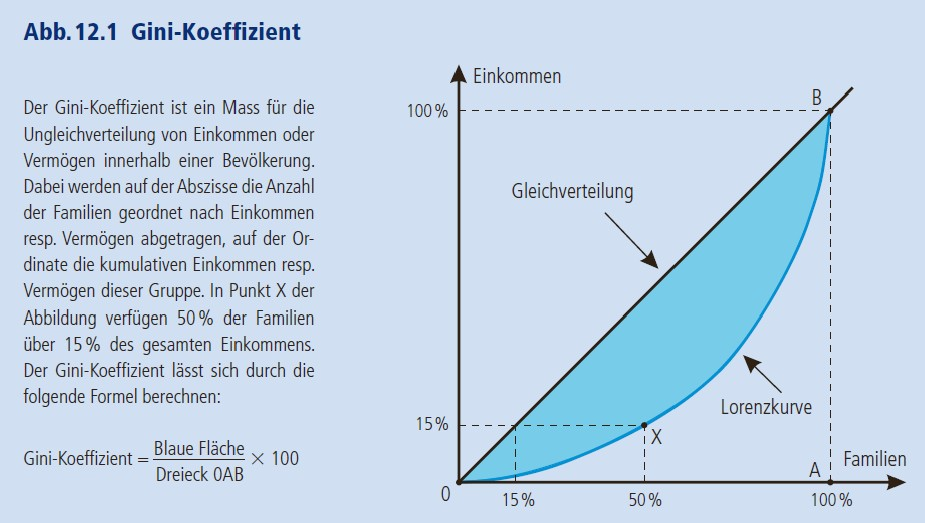
\includegraphics[width=0.8\linewidth]{images/gini.jpg}
\subsection{Umverteilung} 
\begin{multicols}{2}
\textbf{Einkommensquellen}
\begin{itemize}
	\item Lohn
	\item Erträge aus Vermögen
	\item Staatliche Transfers
\end{itemize}
\columnbreak
\textbf{Arten der Umverteilung}
\begin{itemize}
	\item Umverteilung Einnahmen durch progressives Steuersystem (Einnahmeseite)
	\item Verbilligung staatliche Leistungen (Ausgabeseite)
\end{itemize}
\end{multicols}
\subsection{Umverteilung Ausgabenseite: Sozialwerke}
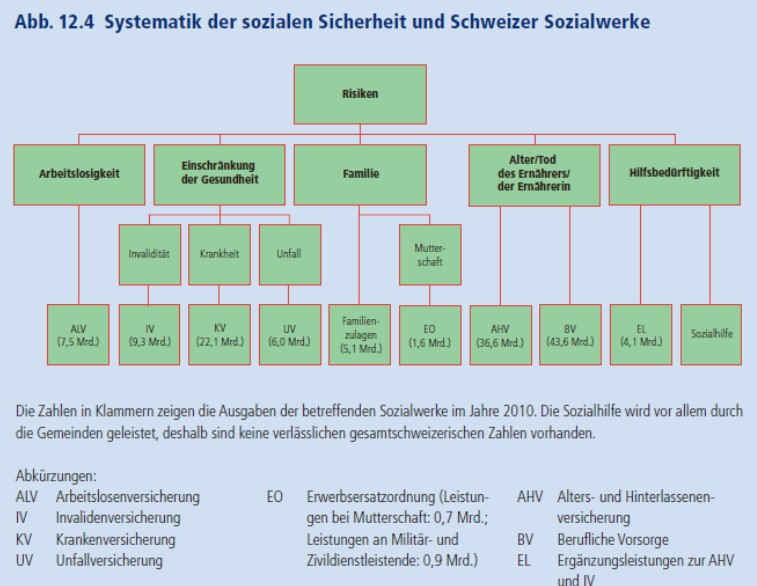
\includegraphics[width=0.8\linewidth]{images/sozialwerke.jpg}
\subsection{Die drei Säulen der Altersvorsorge der Schweiz}
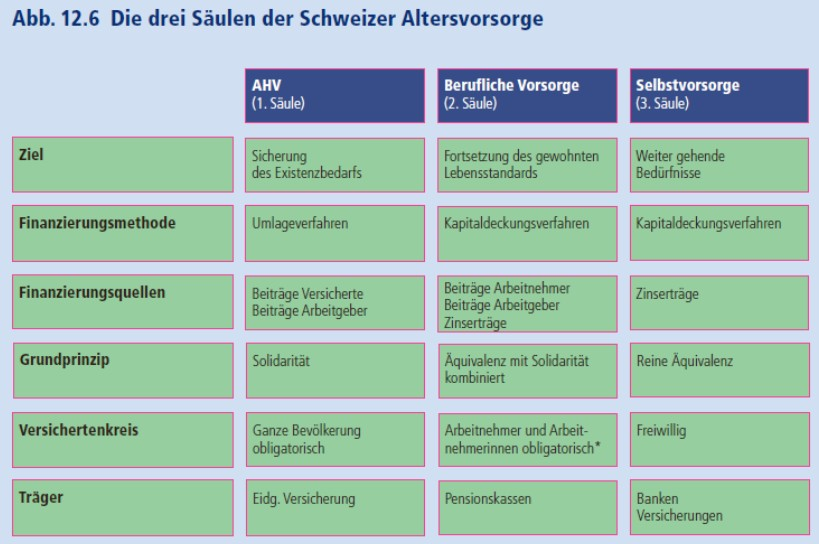
\includegraphics[width=0.8\linewidth]{images/dreisaulen.jpg}
\clearpage
\pagebreak